\chapter{Functions}

\section{Functions, domain, and range}

\begin{figure}
    \centering
    \begin{tikzpicture}
        \draw (0,0) ellipse (1 and 2) node [yshift=30] {domain};
        \draw (5,0) ellipse (1 and 2) node [yshift=30] {codomain};
        \draw (5,0) circle (0.8) node [yshift=10] {range};
        \filldraw (0,0) circle (2pt);
        \filldraw (5,0) circle (2pt);
        \draw [-{Stealth[length=5mm]}] (0,0) -- node [above] {$f$} (5,0);
    \end{tikzpicture}
    \caption{Illustration of the domain, codomain, and range of a function.}
    \label{fig:function_definition}
\end{figure}

\begin{definition}
    A \textbf{function} $f:D\mapsto C$ consists of the following:
    \begin{enumerate}
        \item a set $D$ called the \textbf{domain}, often denoted $\Dom f$,
        \item a set $C$ called the \textbf{codomain},
        \item a rule, that given any point in the domain ($x\in\Dom f$) associates exactly one element $f(x)\in C$.
    \end{enumerate}
    An illustration of a function can be found in Figure \ref{fig:function_definition}.
\end{definition}

For $x\in D$ we write $f(x)$ to denote the assigned element in $C$. This is called the value of $f$ at $x$, or the image of $x$ under $f$, where $x$ is the \textbf{argument} of the function. Extending the above notation:
\[f:D\mapsto C:x\mapsto f(x),\]
which reads as: \emph{f is a function from $D$ to $C$ that associates $x$ in $D$ to $f(x)$ in $C$}.


\begin{definition}
    The \textbf{range} of $f:D\mapsto C$ is the set of all images, that is
    \[\Ran f=\{f(x)\in C:x\in\Dom f\}\]
\end{definition}

\begin{example}
    Say $f:\mathbb R\mapsto\mathbb R$ given by $f(x)=x^2$, $\forall \in\mathbb R$. Here $\Dom{f}=\mathbb R$, $\Ran{f}=[0,\infty)$.
\end{example}

\begin{example}
    Say $f:[0,6]\mapsto\mathbb R:x\mapsto\sqrt{2x+4}$. We know $\Dom{f}=[0,6]$ and $\Ran{f}=[2,4]$.
\end{example}

\begin{example}
    For
    \[f(x)=\dfrac{1}{1-x}\]
    $\Dom{f} = \mathbb R\setminus\{1\}=(-\infty, 1)\cup(1,\infty)$ and $\Ran{f}=\mathbb R\setminus\{0\}$.
\end{example}

The function $f(x)=x^2$ can be defined by the equation $y=x^2$ by using $y=f(x)$, however, not all equations define a function.

\begin{example}
    The equation $y^2=x$ does not define a function $y(x)$ as for $x<0$ there are no real solutions for $y$. There are also two solutions for $y$ for $x>0$ a function must only assign one element of the range for each element of the domain.
\end{example}

\section{The graph of a function}

\begin{definition}
    The \textbf{graph} of a function is a curve in the $(x,y)$ plane, given by
    \[\text{graph\,}f=\{(x,y):x\in\Dom f \text{ and } y=f(x)\}.\]
\end{definition}

A graph over the interval $[a,b]$ is the portion of the graph where the argument is restricted to this interval ($a\leq x\leq b$).

The graph of a function is a curve in the plane, however, not every curve is the graph of a function. The vertical line test determines whether a curve is the graph of a function.

\subsection{The vertical line test}

If any vertical line intersects the curve at more than one point than the curve is not the graph of a function. Otherwise, it is.

\begin{figure}
    \centering
    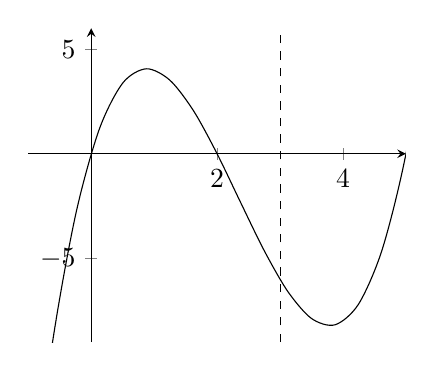
\begin{tikzpicture}
        \begin{axis}[axis lines=middle,
                     xmin=-1, xmax=5, ymin=-9, ymax=6,
                     scale=0.7]
            \addplot[smooth, domain=-1:8] {x * (x - 2) * (x - 5)};
            \addplot[dashed] coordinates {(3,-9) (3,6)};
        \end{axis}
    \end{tikzpicture}
    \begin{tikzpicture}
        \begin{axis}[axis lines = middle,
                     xmin=0, xmax=6, ymin=0, ymax=6,
                     axis equal,
                     scale=0.7]
            \draw (axis cs: 3, 3) circle [radius=2];
            \addplot[dashed] coordinates {(4,0) (4,6)};
        \end{axis}
    \end{tikzpicture}
    \caption{The vertical line text applied to a cubic curve and a circle.}
    \label{fig:vertical_line_example}
\end{figure}

In Figure \ref{fig:vertical_line_example}, the first curve is the graph of the function $f(x)=x(x-2)(x-5)$. We know this is a function as a vertical line will only intersect the graph at one point. The second curve is not the graph of a function as you can draw a vertical line that intersects the curve in two places (as shown). The equation that gives this curve is $(x-3)^2+(y-3)^2=2$.

\begin{figure}
    \centering
    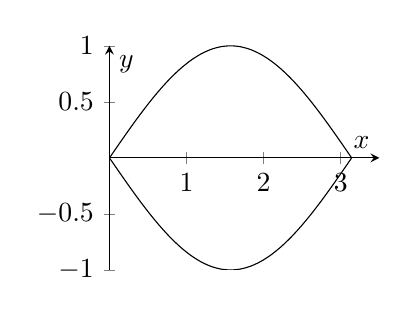
\begin{tikzpicture}
        \begin{axis}[axis lines=middle, scale=0.5, xlabel={$x$}, ylabel={$y$}, xmin=0, xmax=3.5]
            \addplot[smooth, domain=0:3.14] {sin(deg(x))};
            \addplot[smooth, domain=0:3.14] {- sin(deg(x))};
        \end{axis}
    \end{tikzpicture}
    \caption{Curve of $|y|=\sin{x}$}
    \label{fig:modulus_sin_graph}
\end{figure}

\begin{example}
    Use the vertical line test to show whether the equation \[ \abs{y} = \sin{x} \] defines a function.
    
    To draw this curve we ignore all points where $\sin{x}<0$ (as $|y|\geq0$) and we also consider all points for $\sin{x}\geq 0$ reflected on the $x$-axis. This curve is drawn in Figure \ref{fig:modulus_sin_graph}.
\end{example}

\section{Graphs and transformations}

% todo, need to consult lecture notes

\section{Even and odd functions}

\begin{definition}
    A function $f$ is \textbf{even} if
    \[f(-x)=f(x)\quad\forall\pm x\in\Dom f.\]
    The graph of an even function is symmetric under a reflection in the y-axis. 
\end{definition}

\begin{figure}
    \centering
    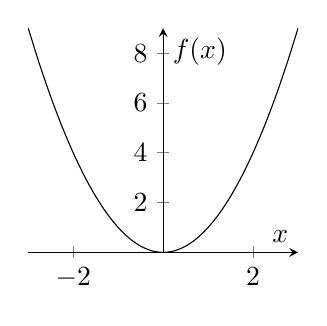
\begin{tikzpicture}
        \begin{axis}[axis lines=middle, xlabel={$x$}, ylabel={$f(x)$}, scale=0.5]
            \addplot[smooth, domain=-3:3] {x^2};
        \end{axis}  
    \end{tikzpicture}
    \caption{Graph of the function $f(x)=x^2$.}
    \label{fig:x_squared_graph}
\end{figure}
    
\begin{example}
    $f(x)=x^2$ is even as $f(-x)=(-x)^2=x^2=f(x)$, it is plotted in Figure \ref{fig:x_squared_graph}.
\end{example}

\begin{definition}
    A function $f$ is \textbf{odd} if
    \[f(-x)=-f(x)\quad\forall\pm x\in\Dom f.\]
    The graph of an odd function i s symmetric under a rotation about the origin of $\pi^c$. This is equivalent to a reflection in the $y$-axis followed by a reflection in the $x$-axis.
\end{definition}

\begin{figure}
    \centering
    \begin{tikzpicture}
        \begin{axis}[axis lines=middle, xlabel={$x$}, ylabel={$f(x)$}, scale=0.8]
            \addplot[smooth, domain=-5:5] {x};
        \end{axis}  
    \end{tikzpicture}
    \caption{Graph of the function $f(x)=x$.}
    \label{fig:x_graph}
\end{figure}

\begin{example}
    $f(x)=x$ is odd as $f(-x)=-x=-f(x)$. The graph of $f$ is shown in Figure \ref{fig:x_graph}.
\end{example}

\begin{theorem}
    All functions $f:\mathbb R\mapsto\mathbb R$ can be written as the sum of an even function and an odd function.
\end{theorem}

\begin{proof}
    Given $f(x)$ let 
    \begin{align*}
        f_{\text{even}}(x)&=\dfrac12\Big(f(x)+f(-x)\Big)\qquad\text{this is even, and}\\
        f_{\text{odd}}(x)&=\dfrac12\Big(f(x)-f(-x)\Big)\qquad\text{this is odd.}
    \end{align*}
    Now,
    \begin{align*}
        f_{\text{even}}(x)+f_{\text{odd}}(x)&=\dfrac12\Big(f(x)+f(-x)+f(x)-f(-x)\Big)\\
        &=f(x)
    \end{align*}
    This is known as proof by explicit construction.
\end{proof}

\begin{example}
    Express the function \[f(x)=(1+x)\sin x\] as the summation of one even and one odd function.
    
    \begin{align*}
        f_{\text{even}}(x)&=\dfrac12\Big((1+x)\sin{x}+(1-x)\sin{(-x)}\Big)\\
        &=\dfrac12(\sin{x}+x\sin{x}-\sin{x}+x\sin{x})\\
        &=x\sin x
    \end{align*}
    \begin{align*}
        f_{\text{odd}}(x)&=\dfrac12\Big((1+x)\sin{x}-(1-x)\sin{(-x)}\Big)\\
        &=\dfrac12(\sin{x}+x\sin{x}+\sin{x}-x\sin{x})\\
        &=\sin{x}
    \end{align*}
    \[f(x)=x\sin{x}+\sin{x}\]
\end{example}

\begin{example}
    Express the function \[f(x)=e^x\] as the summation of one even and one odd function function.
    
    \begin{align*}
        f_{\text{even}}(x)&=\dfrac12(e^x+e^{-x})=\cosh{x}\\
        f_{\text{odd}}(x)&=\dfrac12(e^x-e^{-x})=\sinh{x}\\
        f(x)&=\cosh{x}+\sinh{x}
    \end{align*}
\end{example}

\section{Piecewise functions}

\begin{definition}
    A function is \textbf{piecewise} if it is given by different expression in different parts of the domain.
\end{definition}

\begin{figure}
    \centering
    \begin{tikzpicture}
        \begin{axis}[xlabel = {$x$},
                     ylabel = {$f(x)$},
                     axis lines = middle, 
                     scale = 0.8]
            \addplot[smooth, domain=0:5] {x};
            \addplot[smooth, domain=-5:0] {-x};
        \end{axis}
    \end{tikzpicture}
    \caption{The modulus function, $f(x) = \abs{x}$.}
    \label{fig:modulus_function_graph}
\end{figure}

\begin{example}
    The modulus (or absolute value) is a piecewise function defined by
    \[
        H(x)=
        \begin{cases} 
            x & \text{if }x\geq0\\
            -x & \text{if }x<0
        \end{cases}
        .
    \]
    The graph of the modulus function is shown in Figure \ref{fig:modulus_function_graph}.
\end{example}

\begin{definition}
    A \textbf{step function} is a piecewise function that is constant on each piece.
\end{definition}

\begin{figure}
    \centering
    \begin{tikzpicture}
        \begin{axis}[width=30em, height=15em, xmin=-4, xmax=4, ymin=-0.5, ymax=1.5, xlabel={$x$}, ylabel={$H(x)$}]
            \addplot[domain=-4:0] {0};
            \addplot[domain=0:4] {1};
            \draw[dotted] (axis cs:0,0) -- (axis cs:0,1);
            \addplot[holdot] coordinates{(0,0)(0,1)};
            \addplot[soldot] coordinates{(0,0.5)};
        \end{axis}
    \end{tikzpicture}
    \caption{The Heaviside step function, using the half-maximum convention.}
    \label{fig:heaviside_graph}
\end{figure}

\begin{example}
    The \textbf{Heaviside step function} $H(x)$ is defined by
    \[
        \begin{cases}
            0 & \text{if  }x<0\\
            1 & \text{if }x>0
        \end{cases}
        .
    \]
    In this definition of $H(x)$, $\Dom H=\mathbb R\setminus\{0\}$, because of this there is a half-step convention used in the definition such that $\Dom H=\mathbb R$:
    \[
        H(x)=
        \begin{cases}
            0 & \text{if  }x<0\\
            \frac12 & \text{if }x=1\\
            1 & \text{if }x>0
        \end{cases}
    \]
\end{example}

\section{Operations with functions}

\begin{definition}
    Given functions $f,g$ we can define the following operations:
    \begin{enumerate}
        \item the \textbf{sum} is \[(f+g)(x)=f(x)+g(x)\] with $\Dom{(f+g)}=\Dom f\cap\Dom g$;
        \item the \textbf{difference} is \[(f-g)(x)=f(x)-g(x)\] with $\Dom{(f+g)}=\Dom f\cap\Dom g$;
        \item the \textbf{product} is \[(fg)(x)=f(x)g(x)\] with $\Dom(fg)=\Dom f\cap\Dom g$;
        \item the \textbf{ratio} is \[(\sfrac fg)(x)=\sfrac{f(x)}{g(x)}\] with $\Dom(\sfrac fg)=(\Dom f\cap\Dom g)\setminus\{x\mid g(x)=0\}$; and
        \item the \textbf{composition} is \[(f\circ g)(x)=f(g(x))\] with $\Dom(f\circ g)=\{x\in\Dom g\mid g(x)\in\Dom f\}$.
    \end{enumerate}
\end{definition}

\begin{remark}
    Generally, $f\circ g$ and $g\circ f$ are different functions.
\end{remark}

\begin{example}
    \begin{align*}
        f(x)&=\sin{x}&g(x)&=x^2
    \end{align*}
    \begin{align*}
        (f\circ g)(x)&=f(x^2)\\
        &=sin{(x^2)}\\\\
        (g\circ f)(x)&=g(\sin{x})\\
        &=\sin^2{x}
    \end{align*}
\end{example}

\section{Inverse functions}

\begin{definition}
    A function $f:D\mapsto C$ is \textbf{surjective} if $\Ran{f}=C$, that is \[\forall y\in C\;\exists\,x\in D\mid f(x)=y\]
\end{definition}

\begin{example}
    The following are examples of functions and whether or not they are surjective:
    \begin{enumerate}
        \item $f:\mathbb R\mapsto\mathbb R$, $f(x)=2x+1$ is surjective;
        \item $f:\mathbb R\mapsto\mathbb R$, $f(x)=x^2$ is not surjective; and
        \item $f:\mathbb R\mapsto[0,\infty)$, $f(x)=x^2$ is surjective.
    \end{enumerate}
\end{example}

\begin{definition}
    A function $f:D\mapsto C$ is called \textbf{injective} (one-to-one) if \[\forall x_1,x_2\in D, f(x_1)=f(x_2)\implies x_1=x_2,\] or in other words, $\forall x_1,x_2\in D$ with $x_1\neq x_2$ then $f(x_1)\neq f(x_2)$.
\end{definition}

\begin{example}
The following are examples of functions and whether or not they are injective:
    \begin{enumerate}
        \item $f:\mathbb R\mapsto\mathbb R$, $f(x)=2x+1$ is injective;
        \item $f:\mathbb R\mapsto\mathbb R$, $f(x)=x^2$ is not injective (as $f(1)=1=f(-1)$); and
        \item $f:\mathbb R\mapsto(-\infty,0]$, $f(x)=x^2$ is injective.
    \end{enumerate}
\end{example}

\subsection{The horizontal line test}

If any horizontal line intersects the graph of a function at more than one point then it is not injective, otherwise it is.

\begin{definition}
    A function $f:D\mapsto C$ is \textbf{bijective} if it is both surjective and injective.
\end{definition}

\begin{theorem}[Inverse function theorem]
    A \textbf{bijective} function $f$ has a unique inverse function $f^{-1}$ defined by \[(f^{-1}\circ f)(x)=x=(f\circ f^{-1}).\] To calculate $f^{-1}(x)$, we set $x=f^{-1}(x)$ and $f(x)=x$. Note that
    
    \begin{align*}
        \Dom{f^{-1}}&=\Ran{f};\\
        \Ran{f^{-1}}&=\Dom{f}.
    \end{align*}
\end{theorem}

\section{Elementary functions}

% Check lecture notes for first section todo

\subsection{Rational functions}

\begin{definition}
    A \textbf{rational function} $f$ is the ratio of two polynomials such that
    \[f(x)=\dfrac{p(x)}{q(x)}\]
    where $p(x),q(x)$ are polynomials. The \textbf{simplified form} is obtained by cancelling any common factors in $p$ and $q$. We call a rational function \textbf{proper} if the degree of the top polynomial is less than the degree of the bottom polynomial.
\end{definition}

\begin{example}
    \begin{align*}
        f(x)&=\dfrac{x-1}{x^2-1}\\
        &=\dfrac{(x-1)}{(x-1)(x+1)}\\
        &=\dfrac{1}{x-1}\qquad\text{if }x\neq1
    \end{align*}
    and here $\Dom f=\mathbb R\setminus\{-1,1\}$.
\end{example}

\begin{definition}
    The \textbf{hyperbolic functions} are analogous to the the trigonometric functions, the basic hyperbolic functions are:
    \begin{align*}
        \sinh{x}&=\dfrac12(e^x-e^{-x})\text{; and}\\
        \cosh{x}&=\dfrac12(e^x+e^{-x}).
    \end{align*}
    From these basic functions, the other functions can be derived such as $\tanh{x}$.
\end{definition}

